%\documentclass[t]{beamer}  % [t], [c], или [b] --- вертикальное выравнивание на слайдах (верх, центр, низ)
\documentclass{beamer} % Соотношение сторон

%графики
\usepackage{pgfplots}
\pgfplotsset{compat=1.9}

\usetheme{Madrid}
\usefonttheme{serif}



%%% Работа с русским языком
\usepackage[T2A]{fontenc}			% кодировка
\usepackage[utf8]{inputenc}			% кодировка исходного текста
\usepackage[english,russian]{babel}	% локализация и переносы
%%% Дополнительная работа с математикой
\usepackage{amsmath,amsfonts,amssymb,amsthm,mathtools} % AMS
\usepackage{bm}

%%% Работа с картинками
\usepackage{graphicx}  % Для вставки рисунков
\setlength\fboxsep{3pt} % Отступ рамки \fbox{} от рисунка
\setlength\fboxrule{1pt} % Толщина линий рамки \fbox{}

\usepackage{braket} %Бракеты
\usepackage[version=4]{mhchem} 

\newtheorem{thrm}{Теорема}

\title[]{Определение формы пленки, натянутой между кольцами}

\subtitle{}
\author{Калиничев И.~А.}
\institute[МФТИ]{МФТИ \newline ФОПФ}
\renewcommand{\arraystretch}{1.3}

\setbeamersize{text margin left=20pt,text margin right=20pt}

\usepackage{pgfpages}
%\pgfpagesuselayout{2 on 1}[a4paper,border shrink=5mm]

\begin{document}

\frame[plain]{\titlepage}	% Титульный слайд

\section{проблема}
%%%%%%%%%%%%%%%%%%%%%%%%%%%%%%%%%%%%%%%%%%%%%%%%%%%%%%%%%%%%%%%%%%
%% 2 %%
\begin{frame}[c]
	\frametitle{Постановка задачи}
		\centering
	Между двумя кольцами радиуса R, разведенными на расстояние d, натянута мыльная пленка. Необхожимо определить профиль пленки в приближении $d \ll R$.
\end{frame}
%%%%%%%%%%%%%%%%%%%%%%%%%%%%%%%%%%%%%%%%%%%%%%%%%%%%%%%%%%%%%%%%%%

%% 3 %%
\begin{frame}[c]
	\frametitle{Сведение к матану}
	\centering
	По известной формуле внутренняя энергия пленки $U =  \left( \sigma - T\frac {d\sigma} {dT} \right)F$ пропорциональна ее площади, следовательно пленка примет форму в которой ее площадь минимальна, то есть должен принимать минимум интеграл \[\int_0^1 2 \pi d^2 x(z) \sqrt{1+(x'(z))^2} dz \]
	Здесь были введены обезразмеренные параметры $x(0) = x(1) = \frac {R} {d}, z_{max} = 1$
\end{frame}
%%%%%%%%%%%%%%%%%%%%%%%%%%%%%%%%%%%%%%%%%%%%%%%%%%%%%%%%%%%%%%%%%%

%% 4 %%
\begin{frame}[c]
	\frametitle{Картнка 1}
	\begin{figure}[h]

\centering

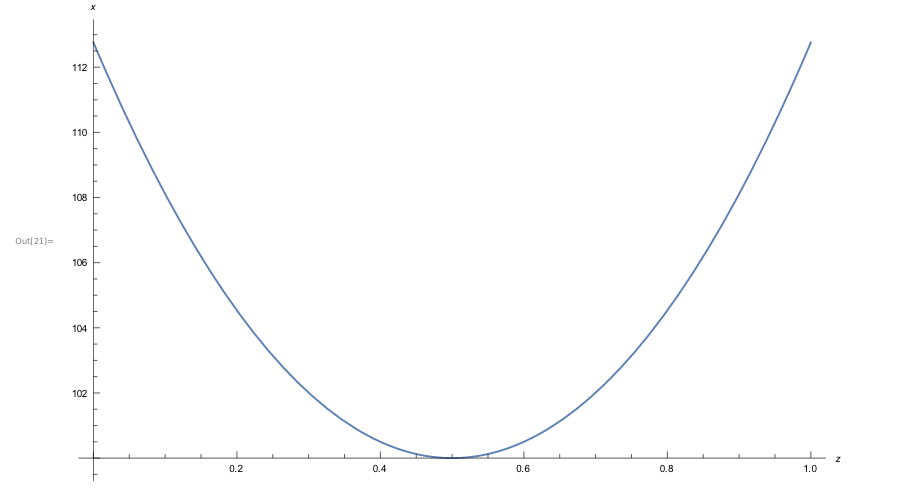
\includegraphics[width=0.8\linewidth]{Kartinka1.png}

\caption{Ожидаемая форма кривой}

\label{fig:mpr}

\end{figure}
\end{frame}
%%%%%%%%%%%%%%%%%%%%%%%%%%%%%%%%%%%%%%%%%%%%%%%%%%%%%%%%%%%%%%%%%%

%% 5 %%
\begin{frame}[c]
	\frametitle{Нахождение x(z)}
	\centering
	\[L(x(z),x'(z)) = x(z) \sqrt{1+(x'(z))^2}\]
	Для того, чтобы функционал принял минимум необходимо, чтобы $\frac{ \partial L(x,x')}{ \partial x} = \frac{d}{ dz}\frac{ \partial L(x,x')}{ \partial x'}$, в итоге получим уравнение \[(x'(z))^2 = x(z) x''(z) -1\] от куда \[x(z) = e^{c_1} ch(e^{-c_1}(z-c_2))\]
\end{frame}
%%%%%%%%%%%%%%%%%%%%%%%%%%%%%%%%%%%%%%%%%%%%%%%%%%%%%%%%%%%%%%%%%%

%% 7 %%
\begin{frame}[c]
	\frametitle{Нахождение констант}
\[\begin{cases}
  x(0) = e^{c_1}ch(e^{-c_1}c_2) = \frac{R}{d} \\
  x(1) = e^{c_1}ch(e^{-c_1}(1-c_2)) = \frac{R}{d}
\end{cases} \]
\[\begin{cases}
  c_2 = \frac{1}{2} \\
  e^{-c_1} = \frac{d}{R}ch(\frac {e^{-c_1}}{2})
\end{cases} \]
	Второе уравнение системы не решается точно, чтобы найти приближенное решение обозначим $e^{-c_1} = \beta$, методом последовательных приближений получим  $\beta_0 = 0,\ \beta_1 = \frac{d}{R},\ \beta_2 = \frac{d}{R}ch(\frac{d}{2R}),\ |\beta_2 - \beta_1| \ll 1 \Rightarrow \beta \approx  \frac{d}{R} + \frac{d^3}{8R^3}$
\end{frame}
%%%%%%%%%%%%%%%%%%%%%%%%%%%%%%%%%%%%%%%%%%%%%%%%%%%%%%%%%%%%%%%%%%

%% 8 %%
\begin{frame}[c]
	\frametitle{Решение уравнения}
	\[x(z) = \left(\frac{d}{R} + \frac{d^3}{8R^3}\right)^{-1} ch \left[ \left(\frac{d}{R} + \frac{d^3}{8R^3}\right)\left(z-\frac{1}{2}\right)\right]\]
		\begin{figure}[h]

\centering

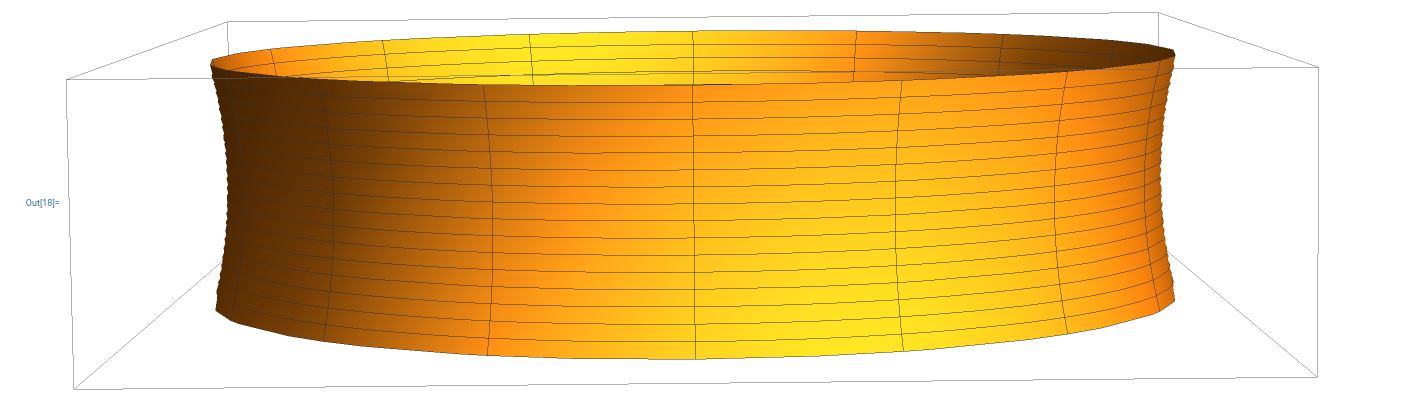
\includegraphics[width=0.8\linewidth]{Kartinka4.png}


\label{fig:mpr}

\end{figure}
		\begin{figure}[h]

\centering

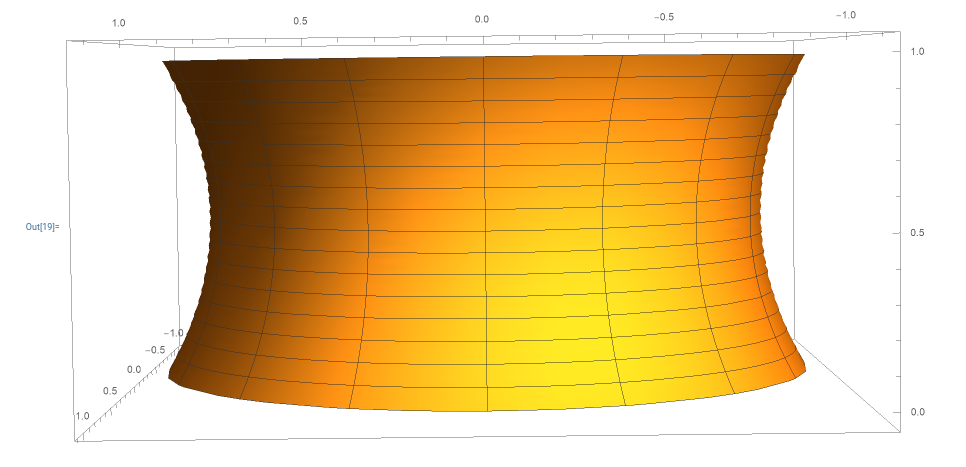
\includegraphics[width=0.5\linewidth]{Kartinka3.png}


\label{fig:mpr}

\end{figure}
\end{frame}
%%%%%%%%%%%%%%%%%%%%%%%%%%%%%%%%%%%%%%%%%%%%%%%%%%%%%%%%%%%%%%%%%%

%% 9 %%
\begin{frame}[c]
	\frametitle{Прогиб} 
	\[P = R - d x\left(\frac{1}{2}\right) = R - \frac{8R^3}{8R^2+d^2} \approx \frac{d^2}{8R} \ll d\]
\end{frame}
%%%%%%%%%%%%%%%%%%%%%%%%%%%%%%%%%%%%%%%%%%%%%%%%%%%%%%%%%%%%%%%%%%

%% 10 %%
\begin{frame}[c]
	\frametitle{}
	\centering
  Спасибо за внимание.
\end{frame}
%%%%%%%%%%%%%%%%%%%%%%%%%%%%%%%%%%%%%%%%%%%%%%%%%%%%%%%%%%%%%%%%%%%%


\end{document}
